\section{Background}

\subsubsection{Apache TinkerPop}

Apache TinkerPop ~\cite{tinkerpop} is a graph computing framework for both graph databases (OLTP) and graph analytic systems (OLAP). It defines a series of basic methods that can be used to interact with a graph: add and remove vertices (resp. edges), retrieve vertex (resp. edges) by an identifier (ID), retrieve vertices (resp. edges) by attribute value, etc. Working only with TinkerPop in an application allows using a graph database in a total implementation-agnostic way, making it possible to easily switch from a graph database to another one without adaptation efforts. 

Apache TinkerPop defines a particular graph model, the property graph, which is basically a directed, edge-labeled, attributed, multi-graph:

\textbf{G = (V, I, VID , D, J, EID , P, Q, R, S)} - (1)
where 
\begin{itemize}
\item V : a set of vertices, 
\item I : a set of vertices identifiers, 
\item VID : V -> I a function that associates each vertex to its identifier, 
\item D : a set of directed edges, 
\item J : a set of edges identifiers, 
\item EID : D -> J a function that associates each edge to its identifier, 
\item P (resp. R) is the vertices (resp. edges) attributes domain and 
\item Q (resp. S) the domain for allowed vertices (resp. edges) attributes values.
\end{itemize}

\subsubsection{Gremlin}

Apache TinkerPop uses the Gremlin graph traversal language to model and analyze the graphs. It also provides a gremlin server which can be configured to use any gremlin-compliant graph databases using the database specific plugin. Clients can be in any programming language and make contacts with the server to execute queries. We use python in this project to access the gremlin server (see fig ~\ref(fig:gremlin)).

Gremlin graph traversal language initially creates a traversal object that gives access to the graph. It then provides five types of steps to operate and transform that traversal. 

\begin{itemize}
\item map - Map the traverser to some object of type E (Can be a vertex, edge, or set of attributes) for the next step to the process
\item flatMap - Map the traverser to some objects of type E (Can be a vertex, edge, or set of attributes) for the next step to the process
\item filter - Map the traverser to either true or false based on a predicate, where false will not pass the traverser to the next step.
\item sideEffect - perform some operation on the traverser (like grouping vertices based on attribute value) and pass it to the next step. 
\item branch - split the traverser to all the traversals indexed by the M token.
\end{itemize}

\begin{figure}[t]
%\vspace{0.2in}
\centering
\resizebox{0.2\linewidth}{!}{
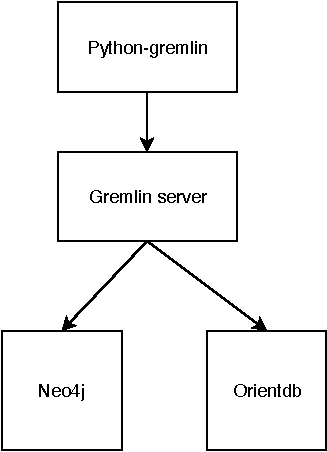
\includegraphics[width=0.8\linewidth]{Images/gremlin.pdf}
}
\caption{Gremlin setup.}
\label{fig:gremlin}
\centering
\end{figure}


Clients query the graph by creating a traversal for a graph and by applying chain of steps on the traversal.

\section{Goal of the study}

The main goal of this study is to empirically compare performance of two most popular open-source graph databases: Neo4j and OrientDB (according to DB ranking~\cite{dbranking}) for pattern-matching queries.

\section{Methodology}

To achieve our goal, we compare performance of graph databases: Neo4j and OrienDB for same pattern matching queries. One approach would be to write the native queries for each database but it would require really good understanding of the native queries and optimization for each database. It would also require expert's opinion to confirm that the pattern matching queries are optimized for each database and then it would be fair to compare the performance of the databases.

Another way to approach this would be to write the pattern-matching queries once and run on both the databases. This would be fair way to compare the databases and also this would be less tedious since we need to learn only one language instead of two as compared to first approach. Tinkerpop framework enables one to write the queries in Gremlin language (designed according to the "write once, run anywhere" philosophy ~\cite{gremlin}). Since both Neo4j and OrientDB are TinkerPop compliant, we implement queries in Gremlin-Python that run on both databases. 

We used the International Movie Database (IMDB) graph available publicly ~\cite{IMDb96:online} for our dataset and pattern-matching queries from the literature ~\cite{tripoulthere} as discussed in the following:  

\subsection{Workload}

\subsubsection{Database}

We use a large real-world IMDB database~\cite{IMDb96:online} with 29,160,968 edges (29 million) and 5,002,524 vertices (5 million). The schema consists of nodes: Movie, Genre,
Actress, Actor and Director. An edge is only possible between a Movie type vertex and a non-Movie type vertex. 
The schema of the database is shown in the figure~\ref{fig:schema}. 

\begin{figure}[t]
%\vspace{0.2in}
\centering
\resizebox{0.3\linewidth}{!}{
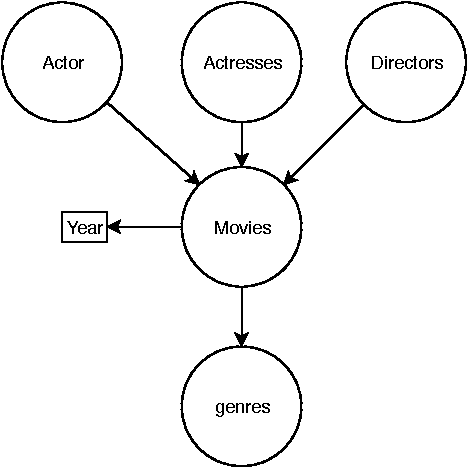
\includegraphics[width=0.8\linewidth]{Images/IMDB_schema}
}
\caption{IMDB database schema.}
\label{fig:schema}
\centering
\end{figure}

\subsubsection{Queries}

We compare the performance of below pattern matching queries when executed with Neo4j or OrientDB as a database. These Queries are implemented in gremlin-python using a multi-threaded approach with each thread searching a particular subset of the graph for the patterns. 

We have to reason for selecting below queries?

\begin{itemize}

\item Pattern 1

The first pattern is to find all persons (actress or actor or director) that worked together on at least 5 different movies.

\begin{figure}[t]
%\vspace{0.2in}
\centering
\resizebox{0.4\linewidth}{!}{
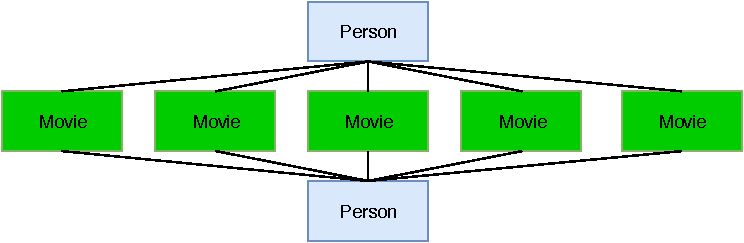
\includegraphics[width=0.8\linewidth]{Images/query1}
}
\caption{Query 1.}
\label{fig:query1}
\centering
\end{figure}

\item Pattern 2

The pattern is to find all persons (actress or actor or director) that worked together on two movies produced in either 2009 or 2011.

\begin{figure}[t]
%\vspace{0.2in}
\centering
\resizebox{0.2\linewidth}{!}{
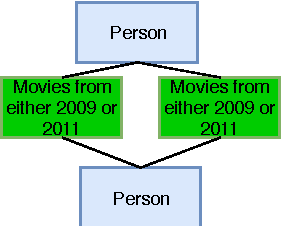
\includegraphics[width=0.8\linewidth]{Images/query2}
}
\caption{Query 2.}
\label{fig:query2}
\centering
\end{figure}

\item Pattern 3

The pattern is to find all persons (actress or actor or director) that worked in at least 5 different movies that fall under a similar genre.


\begin{figure}[t]
%\vspace{0.2in}
\centering
\resizebox{0.4\linewidth}{!}{
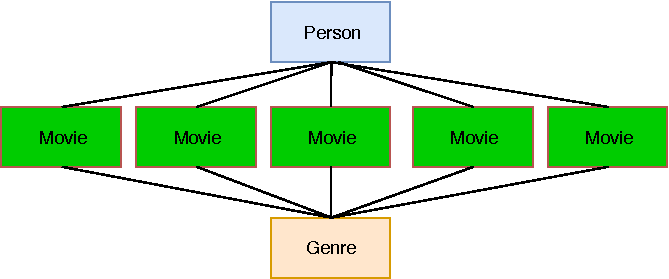
\includegraphics[width=0.8\linewidth]{Images/query3}
}
\caption{Query 3.}
\label{fig:query3}
\centering
\end{figure}

\item Pattern 4

The first pattern is to find all actresses, actors, and directors that worked together on at least three different movies.


\begin{figure}[t]
%\vspace{0.2in}
\centering
\resizebox{0.3\linewidth}{!}{
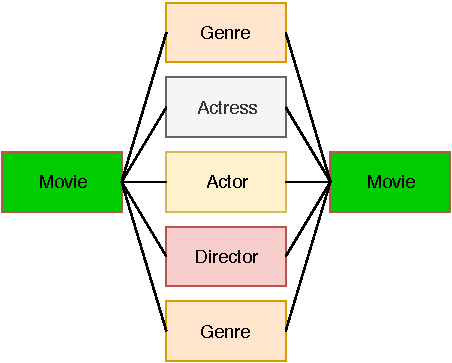
\includegraphics[width=0.8\linewidth]{Images/query4}
}
\caption{Query 4.}
\label{fig:query4}
\centering
\end{figure}

\item Pattern 5

The pattern is to find all actresses, actors, and directors that worked together on two movies produced in 2009 and 2011 respectively.


\begin{figure}[t]
%\vspace{0.2in}
\centering
\resizebox{0.3\linewidth}{!}{
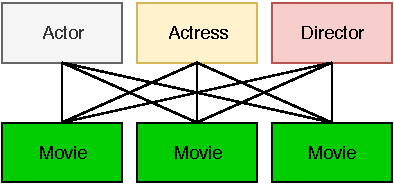
\includegraphics[width=0.8\linewidth]{Images/query5}
}
\caption{Query 5.}
\label{fig:query5}
\centering
\end{figure}

\item Pattern 6

The pattern is to find all the actresses, actors, and directors that worked together at least in two different movies that fall under a similar genre.


\begin{figure}[t]
%\vspace{0.2in}
\centering
\resizebox{0.3\linewidth}{!}{
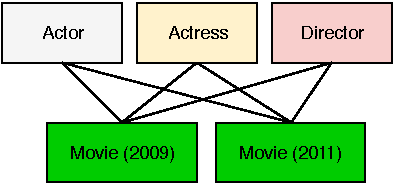
\includegraphics[width=0.8\linewidth]{Images/query6}
}
\caption{Query 6.}
\label{fig:query6}
\centering
\end{figure}

\end{itemize}
